\begin{example}~
\label{ex:single_channel}
	Consider a case where the set of confidential information is represented as $P = \set{(1,3),(2,1),(3,4),(4,1),(5,5),(6,9)}$. Suppose that \AgentOne sends this information encrypted over a single communication channel as $Q = \set{(1,12),(2,1),\\(3,16),(4,1),(5,17),(6,18)}$. \newline 
	
	We define the relations $P$ and $Q$ in \relview\ as follows: \newline
	
	\begin{figure}[ht]
		\centering
		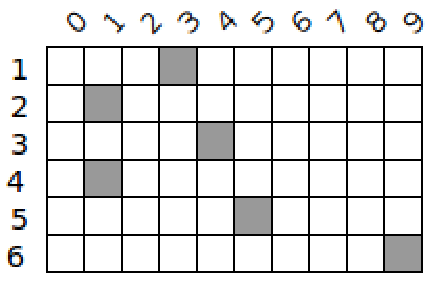
\includegraphics[scale=0.65]{Figures/PDF/Relview/P.pdf}
		\caption{Relation $P$ for Example~\ref{ex:single_channel}.}
		\label{fig:single_channel_p}
	\end{figure}
	
	\begin{figure}[ht]
		\centering
		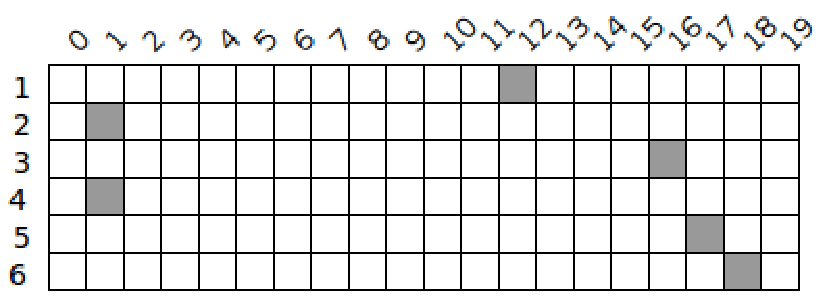
\includegraphics[scale=0.65]{Figures/PDF/Relview/Q.pdf}
		\caption{Relation $Q$ for Example~\ref{ex:single_channel}.}
		\label{fig:single_channel_q}
	\end{figure}	
	
	We verify the existence of an abstraction relation by applying Corollary~\ref{cor:test} using \relview. By executing Program~\ref{prog:test} ($Result = Test(P,Q)$), we obtain the following result: \newline
	
	\begin{figure}[ht]
		\centering
		
\includegraphics[scale=0.65]{Figures/PDF/Relview/True.pdf}
		\caption{Relation $Result$ for Example~\ref{ex:single_channel}.}
		\label{fig:single_channel_result}
	\end{figure}

	Therefore, the test has passed meaning that there exists an abstraction relation relating the confidential information to the information observed to be sent on the communication channel. This means that we can apply Corollary~\ref{cor:compute} by executing Program~\ref{prog:compute} ($X = Compute(P,Q,\RAtop)$) to obtain the abstraction relation, $X$. \newline

	\begin{figure}[ht]
		\centering
		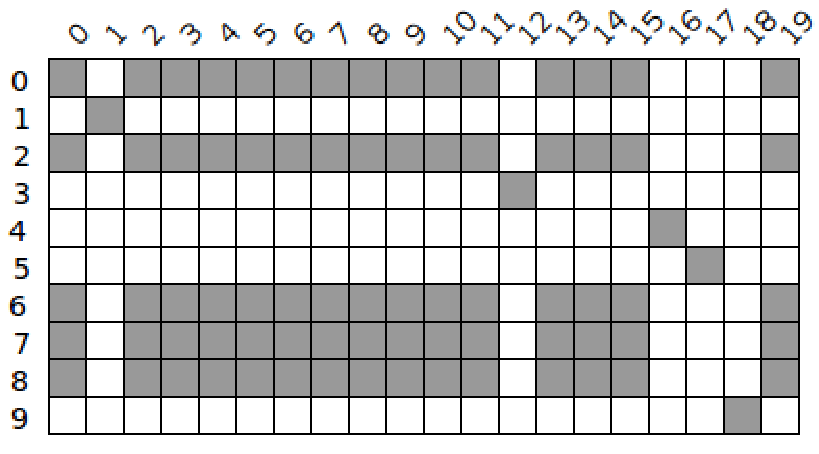
\includegraphics[scale=0.65]{Figures/PDF/Relview/X.pdf}
		\caption{Abstraction relation $X$ for Example~\ref{ex:single_channel}.}
		\label{fig:single_channel_x}
	\end{figure}

	From this result, we can see that there are some digits which are related to information which we do not necessarily have an interest in, \ie we are only concerned with the confidential information which consists of the digits $1,3,4,5, \text{ and } 9$. Therefore we can design a filter $R$ which can be used to refine the abstraction relation $X$. We define $R$ in \relview\ as follows: \newline
	
	\begin{figure}[ht]
		\centering
		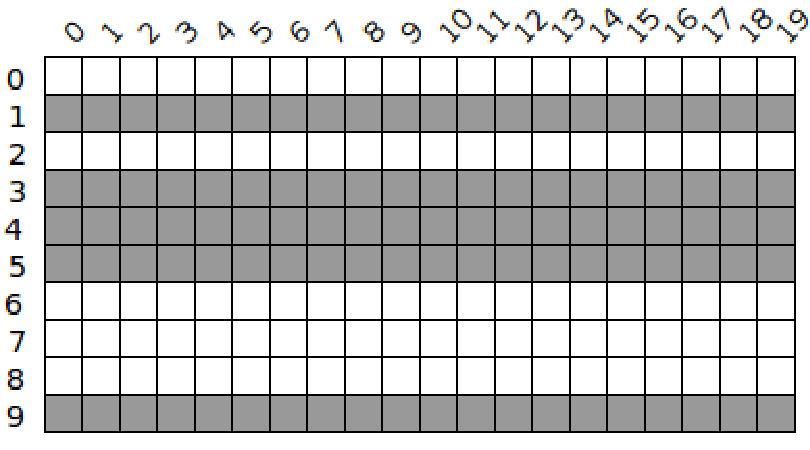
\includegraphics[scale=0.65]{Figures/PDF/Relview/R.pdf}
		\caption{Filtering relation $R$ for Example~\ref{ex:single_channel}.}
		\label{fig:single_channel_r}
	\end{figure}
	
	By executing Program~\ref{prog:compute} with the filter $R$, ($X_{filtered} = Compute(P,Q,R)$), we obtain the abstraction relation, $X_{filtered}$ \newline
	\vspace{-0.25in}
	\begin{figure}[ht]
		\centering
		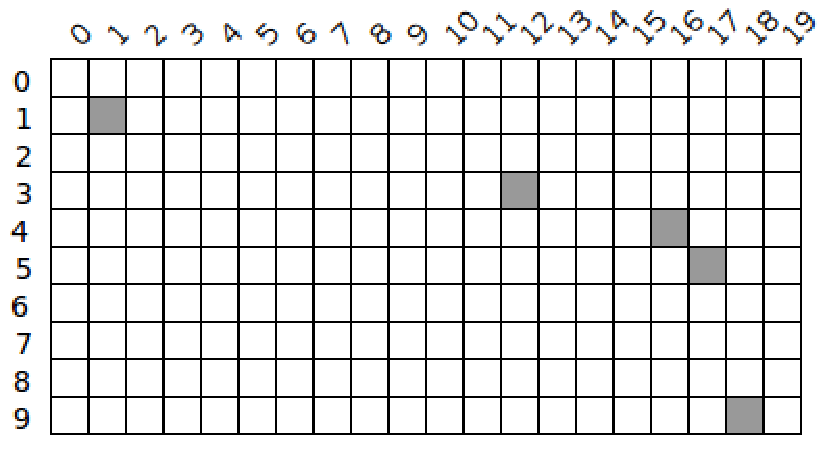
\includegraphics[scale=0.65]{Figures/PDF/Relview/XR.pdf}
		\caption{Abstraction relation $X_{filtered}$ for Example~\ref{ex:single_channel}.}
		\label{fig:single_channel_xr}
	\end{figure}
	 
\end{example}